\documentclass{article}

\usepackage{rotating}
\usepackage{graphicx}
\usepackage[utf]{inputenc}
\usepackage{url}


\title{Industrial Best Practice}


\begin{document}


\author{John Burchell \qquad William Granli \\
		john.a.burchell@gmail.com \qquad william.granli@gmail.com \\
		Computer Science and Engineering  \\
		University of Gothenburg }



\maketitle
\section{Executive Summary, 1p}
Do this last! 

\url{http://unilearning.uow.edu.au/report/4bi1.html}

\section{Problem Formulation, 3p}

\begin{itemize}
	\item Description of what problem you are trying to solve
	\item The description should highlight why the problem is important, for whom it is important and how it advances the state of the art/company business
	\item Description of similar solutions available for the market
\end{itemize}



\section{Plan and Roadmap, 5p}
As mentioned in Section 2, the effects mo ifications to APIs have on the platform’s ecosystem are explored as being negative. However, there are no existing systematic guidelines or framewor s that take the ecosystem into account for how to best modify an API. Our proposed process for creating such a framework will be can be seen in Figure \ref{fig:roadmap}. This is an initial version of the roadmap \cite{!!!roadmap}, and it is advised that it is updated dur ng the process. The main reason for this is that it is impo tant to adapt to changes in the market, and if new needs are identified, the strategy should be redesigned to meet them. 

\subsection{Designing the Roadmap}
The roadmap was developed using the standard T-Plan process \cite{!!!roadmap}. As such, identifying the market need was done as a part of the initial step. Following that, the products and technology needed to fill that gap were identified. As a final step the dependencies and ordering of the identified activites were sorted out which resulted in the current version of the roadmap. An overview of the process used to create the roadmap can be seen in Table \ref{tab:proc}

\begin{table}[ht]
\centering
\begin{tabular}[ht]{|c|l|l|}
\hline
\textbf{\#} & \textbf{Phase} & \textbf{Description} \\
\hline
1 & External & Identify the market needs \\
\hline
2 & Products & Identify required studies \& frameworks \\
\hline
3 & Technology & Identify required knowledge \\
\hline
4 & Organize & Identify what pull factors require which push factors \\
\hline
\end{tabular}
\caption{Roadmap Design Process}
\label{tab:proc}
\end{table}

\subsection{Knowledge Development}
Since we have made the assessment that the market need will remain relatively stable, careful research is essential to be able to deliver a product that meets the market needs. The main way of performing the initial study, to be able to increase the knowledge, will be through studying the existing literature. The reason for this is that three fields (API design, software evolution and software ecoystems) are currently well-explored, but the correlation and relationship between them has not yet been identified. Therefore, these fields will be explored in literature and a set of ``best practices" will be gathered from each field. 

In addition to the literature review, a case study will be conducted to gather information from a state of the art company. The goal of the data collection made in the case study, will also be to gather a set of best practices for each of the three fields. This will be achieved by analysing the changes between two versions of the company's platform API. 


\subsection{Implementing the Framework}
To be able to create a framework which uses as much as possible of the knowledge and technology that exists in the world, the results from the literature review and the case study will both be analysed and compared. A set of best practices based on both data collections will be defined and become the basis for the framework. That we bring in important factors from each of the three fields in the discussion is of the highest importance. The goal of this phase is to create an Minimum Viable Product (MVP) that can be adopted and evaluated at the case company. 

\subsection{Adoption and Evaluation}
The final stage of the roadmap will take a more iterative approach, where the MVP will be continuously evaluated and improved at the case company. The main way of evaluating the success of the framework will be to measure if there is an decrease in the negative effects that the API has on its ecosystem, while it still is able to remain its original complexity and usability. 


\begin{sidewaysfigure}[p]
\centering
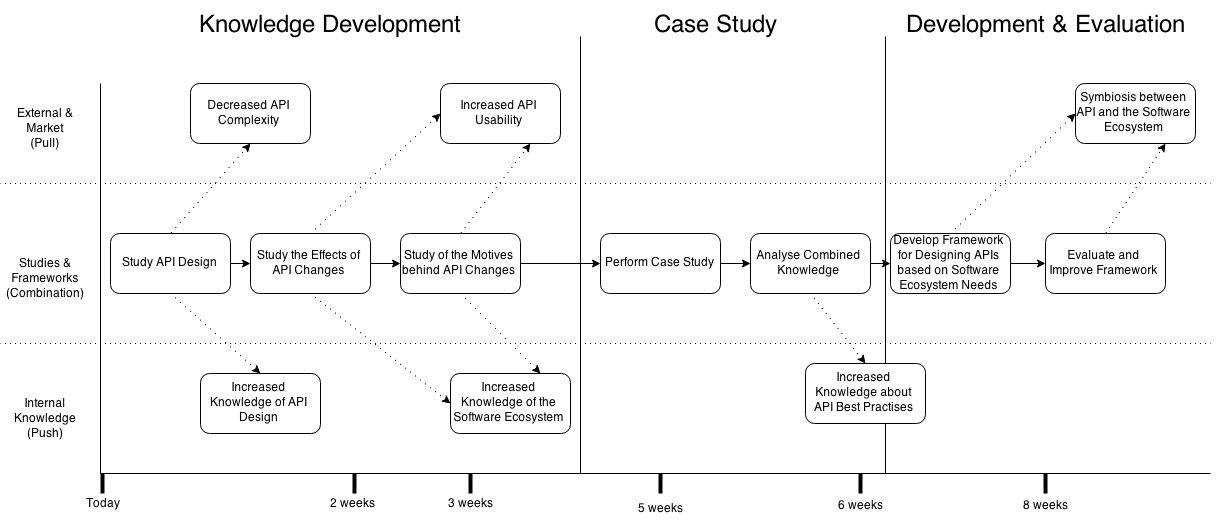
\includegraphics[width=220mm]{RoadMap.png}
\caption{The full lines denote in which way the organisation should ``logically'' view the roadmap. The dotted lines denote that one activity will lead to another. }
\label{fig:roadmap}
\end{sidewaysfigure}
%TODO: Add colours+graphix so that it's innovative and stuff

\section{Dissemination Plan, 2p}

\begin{itemize}
	\item Description on how to present/sell the solution to the company
	\item Description on how to communicate the solution
\end{itemize}

\url{http://www.webarchive.org.uk/wayback/archive/20140614222502/http://www.jisc.ac.uk/fundingopportunities/projectmanagement/planning/dissemination.aspx}

\section{Impact Assessment, 2p}


\begin{itemize}
	\item Description of how the solution advances the state of the art
	\item Description of how the solution advances the society in general (e.g. better cars, faster mobiles)
\end{itemize}

\url{http://en.wikipedia.org/wiki/Impact_assessment}


\section{Summary, 1p}

\begin{itemize}
	\item Account of how you can use the knowledge from the course in your further work
\end{itemize}




\end{document}